% vim: set textwidth=78 autoindent:

\subsection{Plugin Convertitore Dxf2Shp}

% when the revision of a section has been finalized, 
% comment out the following line:
%\updatedisclaimer

Il plugin Convertitore dxf2shape permette di convertire i dati vettoriali dal formato DXF al formato Shape. È molto semplice da maneggiare e offre la seguente funzionalità come mostrato in Figura \ref{fig:dxf2shape_dialog}.

\begin{itemize}
\item \textbf{File DXF in Input}: Scrivere il percorso del file DXF da convertire
\item \textbf{Output file}: Scrivere il nome che si desidera attribuire al file Shape che verrà creato
\item \textbf{Tipo di file in output}: Specifica il tipo di file in output. Al momento sono supportati i tipi: polilinea, poligono e punto.
\item \textbf{Esporta le etichette di testo}: Se si seleziona questa casella, viene creato un layer di punti in forma di file Shape aggiuntivo, e la tabella dbf associata conterrà informazioni circa i campi "TESTO" trovati nel file dxf e le stringhe di testo propriamente dette.
\end{itemize}

\begin{figure}[ht]
   \begin{center}
   \caption{Plugin Convertitore Dxf2Shape \nixcaption}\label{fig:dxf2shape_dialog}\smallskip
   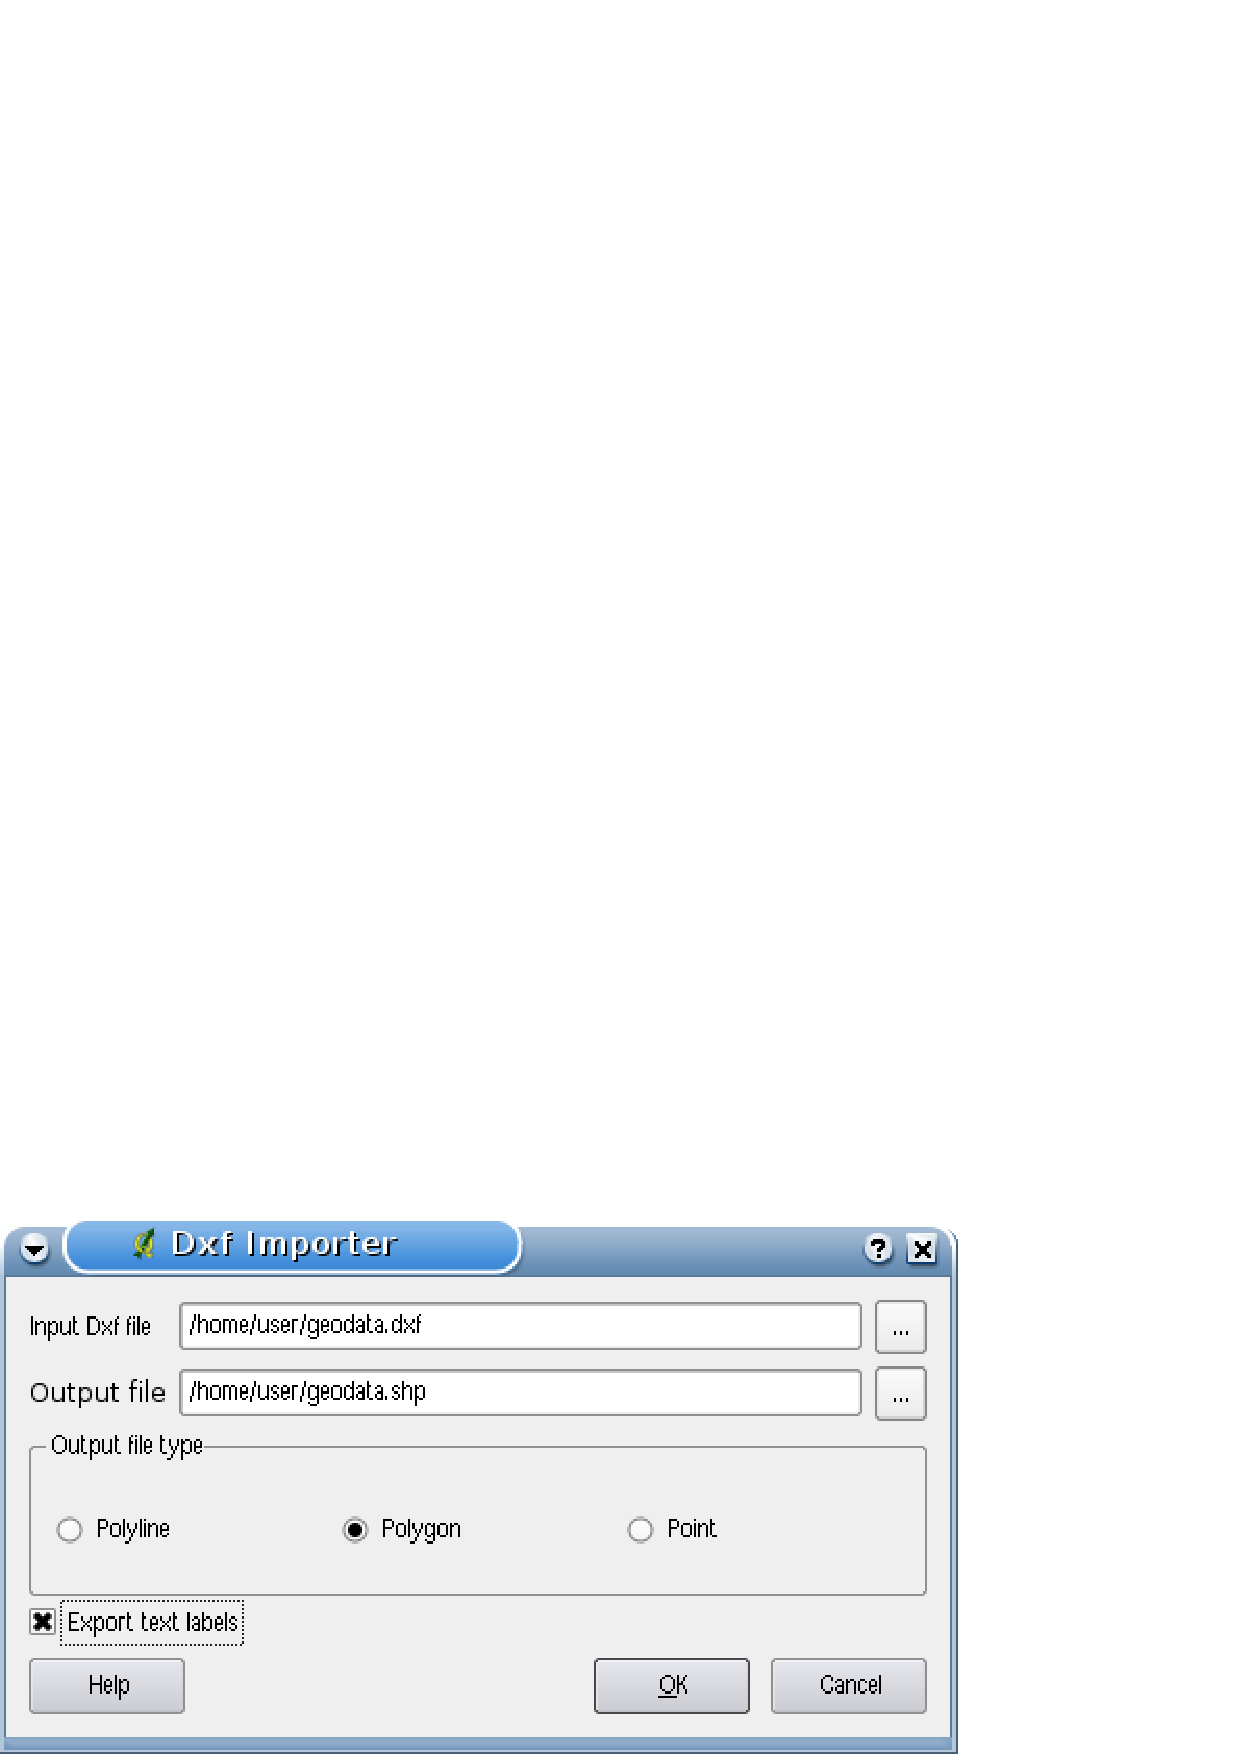
\includegraphics[clip=true, width=13cm]{dxf2shape_dialog}
\end{center}
\end{figure}

\begin{enumerate}
  \item Avviare QGIS, caricare il plugin Dxf2Shape nel Gestore dei Plugins (Vedere Sezione \ref{sec:load_core_plugin}) e premere l'icona \toolbtntwo{dxf2shp_converter}{Convertitore Dxf2Shape} che compare nel menu della barra degli strumenti di QGIS. La finestra di dialogo del plugin Dxf2Shape appare come mostrato in Figura \ref{fig:dxf2shape_dialog}.
  \item introdurre il file DXF in Input, un nome per il file Shape in Output ed il tipo di file Shape.
  \item Abilitare la casella \checkbox{Esporta le etichette di testo}, se si vuole creare un layer addizionale di punti con le etichette.
  \item Premere \button{Ok}. 
\end{enumerate}

\newpage



